\scanpage{15}
\mspage{6}

diagonales de l'hexagone, ou encore aux
trois pts d'ordre $2$ distincts de $e$.

Ici encore on peut ``doubler'' la
décomposition cellulaire, et en \unsure{tirer|trouve}
une autre avec $4$ sommets, \deleted{\unsure{8|6}}\inserted{12} arêtes,
et $8$ faces (triangulaires), qui permet
de mieux comprendre le passage
au quotient par $\pm1$, avec
quatre sommets (dont un sommet
privilégié, correspondant \unsure{:|à} $e$),

\figure{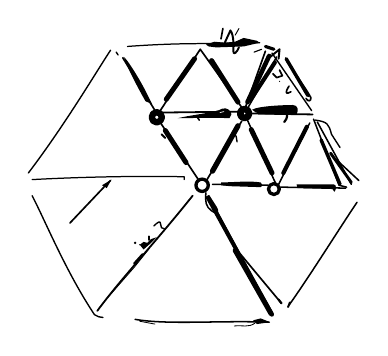
\begin{tikzpicture}[x=.012cm,y=-.012cm,line cap=round,line join=round] \draw[line width=.5pt] (110,48) .. controls (93,74) and (61,128) .. (23,178); \draw[line width=.45pt] (128,44) .. controls (155,42) and (181,41) .. (206,41) -- (268,40); \draw[line width=.45pt] (27,185) .. controls (82,182) and (144,181) .. (188,182) -- (188,185); \draw[line width=.5pt] (27,202) .. controls (41,229) and (63,283) .. (93,328) .. controls (96,330) and (99,331) .. (102,331); \draw[line width=.65pt] (96,324) .. controls (121,290) and (158,251) .. (197,202); \draw[line width=.3pt] (107,310) -- (135,278) -- (151,258); \draw[line width=.55pt] (371,209) .. controls (349,242) and (321,287) .. (299,318); \draw[line width=.7pt] (298,320) -- (300,315); \draw[line width=.55pt] (136,333) .. controls (171,339) and (225,334) .. (278,336); \draw[line width=.3pt] (141,335) -- (157,338); \draw[line width=.3pt] (241,340) .. controls (250,339) and (256,342) .. (263,337); \fill (261,334) -- (269,332) -- (279,336) -- (265,338) -- cycle; \draw[line width=.5pt] (116,50) -- (118,53); \draw[line width=.6pt] (123,56) -- (159,115); \fill (124,55) .. controls (129,59) and (144,84) .. (150,97) -- (154,105) -- (147,102) .. controls (138,86) and (128,67) .. (124,55) -- cycle; \draw[line width=.6pt] (162,113) -- (205,47) -- (250,110); \draw[line width=1.8pt] (169,100) -- (199,57); \draw[line width=1.8pt] (217,59) -- (245,103); \draw[line width=.6pt] (163,125) -- (203,185); \draw[line width=1.8pt] (168,133) -- (190,167); \draw[line width=.65pt] (164,137) -- (168,141); \draw[line width=.6pt] (211,187) -- (249,123); \draw[line width=1.9pt] (218,176) -- (245,128); \draw[line width=.5pt] (241,138) -- (243,139) -- (244,145); \draw[line width=.65pt] (164,114) -- (248,113); \fill (181,120) .. controls (198,116) and (222,114) .. (228,110) .. controls (233,108) and (238,112) .. (238,116) -- (236,120) .. controls (216,119) and (196,120) .. (181,120) -- cycle; \draw[line width=.6pt] (202,119) -- (204,122); \draw[white,line width=.25pt] (226,114) -- (230,113); \draw[line width=.6pt] (253,108) -- (274,49); \draw[line width=1.65pt] (255,103) -- (278,54); \draw[line width=.55pt] (256,108) -- (286,55); \draw[line width=1.5pt] (258,101) -- (284,61); \draw[line width=.7pt] (278,56) -- (289,47) -- (288,57); \draw[line width=1.15pt] (274,44) -- (283,47); \draw[line width=.4pt] (270,47) -- (262,50); \draw[line width=.5pt] (281,51) -- (323,112); \draw[line width=1.25pt] (296,57) -- (319,96); \draw[line width=.6pt] (297,60) .. controls (300,65) and (318,90) .. (322,98) .. controls (323,102) and (319,103) .. (317,99); \draw[line width=.6pt] (289,69) -- (292,75) -- (286,77) -- (282,73); \draw[line width=.6pt] (299,86) .. controls (294,94) and (296,95) .. (301,92); \fill (289,81) circle[radius=.7]; \draw[line width=.65pt] (259,115) -- (324,116); \fill (260,111) .. controls (266,107) and (295,106) .. (303,106) .. controls (309,106) and (309,112) .. (307,116) -- (275,116) -- (264,114) -- cycle; \draw[line width=.8pt] (297,115) .. controls (297,120) and (296,122) .. (294,124); \draw[line width=.55pt] (255,122) -- (283,185) -- (285,189); \draw[line width=1.8pt] (259,132) -- (281,178); \draw[line width=.55pt] (288,190) -- (321,125); \draw[line width=1.5pt] (293,178) -- (318,129); \draw[line width=.55pt] (325,121) -- (352,191) -- (360,193); \draw[line width=1.25pt] (333,143) -- (353,190); \draw[line width=.55pt] (329,124) -- (365,190); \draw[line width=1.05pt] (343,157) -- (365,188); \draw[line width=.55pt] (345,160) -- (373,186); \draw[line width=.5pt] (327,122) .. controls (340,124) and (341,126) .. (344,137) -- (353,151); \draw[line width=.55pt] (218,190) -- (277,191); \fill (227,188) .. controls (239,188) and (257,186) .. (269,188) -- (271,191) -- (269,193) -- (237,192) -- (227,191) -- cycle; \draw[line width=.55pt] (290,193) -- (359,194); \fill (307,190) -- (346,190) .. controls (350,190) and (349,196) .. (347,198) -- (345,195) -- (308,194) -- cycle; \draw[line width=.55pt] (211,199) .. controls (210,208) and (211,214) .. (217,218) .. controls (224,223) and (225,219) .. (221,213) -- (214,202); \draw[line width=1.45pt] (213,204) -- (281,328); \draw[line width=1.8pt] (242,260) -- (280,327); \draw[line width=.6pt] (218,210) -- (246,262) -- (291,316); \draw[line width=.8pt] (288,312) -- (291,316); \draw[line width=.6pt] (67,231) -- (103,193) -- (110,186); \fill (101,191) -- (111,185) -- (106,194) -- cycle; \draw[line width=.8pt] (135,274) -- (144,264); \fill (141,254) -- (145,259) -- (153,252) -- (159,246) -- (153,248) -- (149,252) -- (145,251) -- cycle; \draw[line width=.55pt] (151,249) -- (151,245); \fill (136,252) circle[radius=1.4]; \fill (141,254) circle[radius=.6]; \draw[line width=.5pt] (156,234) .. controls (160,230) and (163,228) .. (163,232) -- (164,236) -- (167,237); \fill (211,42) -- (220,39) -- (231,40) -- (242,39) -- (251,35) -- (265,38) -- (268,40) -- (251,44) -- (222,45) -- (214,44) -- cycle; \draw[line width=.6pt] (227,36) -- (229,25); \draw[line width=.7pt] (231,40) -- (237,27) .. controls (241,33) and (240,43) .. (240,49) .. controls (240,54) and (244,50) .. (246,45); \draw[line width=.35pt] (242,32) -- (246,25); \draw[line width=2.3pt] (159,119) circle[radius=5.4]; \draw[line width=2.4pt] (252,115) circle[radius=4.8]; \draw[line width=1.2pt] (207,191) circle[radius=6.5]; \draw[line width=1.2pt] (283,195) circle[radius=5.8]; \end{tikzpicture}}

six ar\unsure{ê|e}tes les reliant $2:2$ : c'est la
structure tétraédrale \inserted{(orientée)}, avec un sommet
fixé, groupe \unsure{d'automorphismes|d'automorphisme} $\mathbb Z/3\mathbb Z$
(\deleted{\unsure{pourtant}} $\simeq\mathbb Z/6\mathbb Z\,/\pm1$, OK !).

\margin{14}
